\input{../header.tex}

\subject{VERSUCH NUMMER 203}
\title{Verdampfungswärme und Dampfdruck-Kurve}
\date{
  Durchführung: DATUM
  \hspace{3em}
  Abgabe: DATUM
}

\begin{document}

\maketitle
\thispagestyle{empty}
\tableofcontents
\newpage
\setcounter{page}{1}
\section{Ziel}
\label{sec:Ziel}

In diesem Versuch wird der Umgang mit einem Diodenlaser geübt. Dazu wird sowohl die Fluoreszenz sichtbar gemacht, 
als auch das Spektrum von Rubidium aufgenommen.
\section{Theorie}
\label{sec:Theorie}

\subsection{Besetzungsinversion}


\subsection{p- und n-Dotierung}


\subsection{Diodenlaser}
Der Diodenlaser besteht aus einem Halbleiter-Chip, der in \autoref{fig:LaserChip} 
dargestellt ist.
\begin{figure}
    \centering
    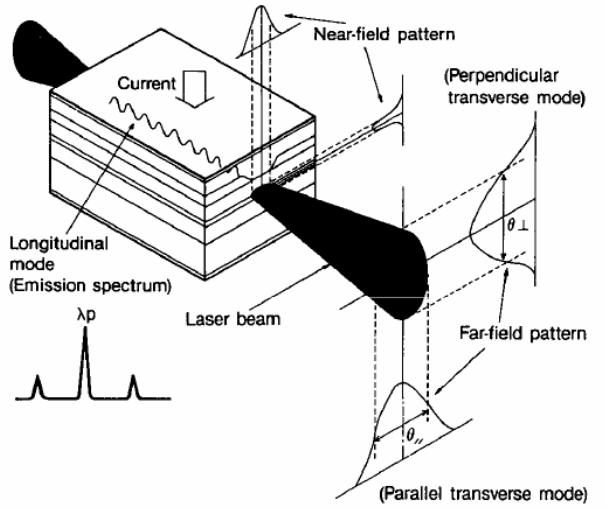
\includegraphics[width=0.8\textwidth]{LaserChip.png}
    \caption{Schematischer Aufbau eines Diodenlaser-Chips \cite{ap60}.}
    \label{fig:LaserChip}
\end{figure}
Dieser besteht aus einer p-dotierten und einer n-dotierten Schicht. Der Übergang 
dazwischen, der pn-Übergang, ist das aktive Medium. An einem der langen Enden befindet sich ein 
undurchlässiger Reflektor, an der gegenüberliegenden Seite ein halbdurchlässiger Reflektor. Dies wird über 
eine Polierung der Seiten realisiert. Auf der halbdurchlässigen Seite kann das verstärkte Laserlicht austreten.
\\
\\
Der Chip ist Teil der Littrow-Konfiguration, die in \autoref{fig:Littrow} abgebildet ist. 
\begin{figure}
    \centering
    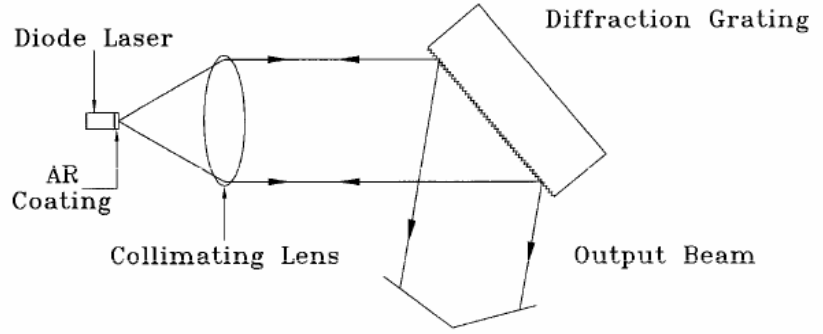
\includegraphics[width=0.8\textwidth]{LittrowSetup.png}
    \caption{Schematischer Aufbau des Laser-Systems (Littrow-Konfiguration) \cite{ap60}.}
    \label{fig:Littrow}
\end{figure}
Außerhalb des Chips befinden sich eine Kollimator-Linse, die den Laserstrahl zu einer 
parallelen Welle macht, und ein Beugungsgitter. Wenn die Welle auf das Gitter trifft, wird 
das nullte Maximum aus dem Laser hinaus gelenkt, während das Maximum erster Ordnung zurück in den 
Laser reflektiert wird. Dessen Wellenlänge wird durch 
\begin{equation*}
    \lambda = 2dsin(\theta)
\end{equation*}
festgelegt, wobei d die Gitterkonstante und $\theta$ der Winkel des Gitters sind. Es bildet sich 
eine weitere stehende Welle zwischen dem Gitter und dem undurchlässigen Reflektor am anderen Ende des 
Chips aus. Dies nennt man auch den externen Resonator.

\subsection{Nettoleistung der verschiedenen Bauteile}
In \autoref{fig:Gain} wird die Nettoleistung des internen und externen Resonators sowie des Gitters in Abhängigkeit von der Wellenlänge dargestellt. 
Außerdem wird die Nettoleistung ohne zusätzliche Bauteile abgebildet. Die einzelnen Kurven sind relativ zueinander dargestellt.
\begin{figure}
    \centering
    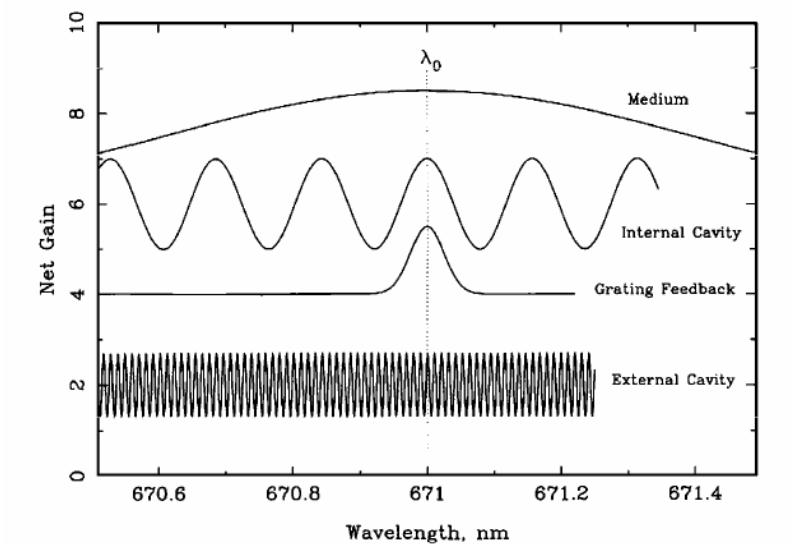
\includegraphics[width=0.8\textwidth]{NetGain.png}
    \caption{Beiträge verschiedener Bauteile zur Nettoleistung \cite{ap60}.}
    \label{fig:Gain}
\end{figure}
Die im aktiven Medium emittierte Strahlung hat ein breites Spektrum mit einem Maximum bei der Wellenlänge 
$\lambda$, die über die Bandlücke bestimmt wird. Die Energie der Bandlücke entspricht 
\begin{equation*}
    E = \frac{\symup{hc}}{\lambda} \, \, ,
\end{equation*}
wobei h das Plancksche Wirkungsquantum ist. Das breite Spektrum ergibt sich dadurch, dass die Elektronen sich in Bändern
befinden und nicht auf diskreten Niveaus. So höher ein Elektron im Leitungsband liegt, desto höher ist dessen Energie.
Das Gitter hat sein Maximum in der Nullten Ordnung, welches als einziges aus dem Laser emittiert wird. Alle weiteren Ordnungen werden
in andere Richtungen gestreut und haben so keinen Einfluss auf die Nettoleistung des Laserstrahls. 
Aus diesem Grund ergibt sich ein Peak bei einer einzigen Wellenlänge.
Der innere Resonator verstärkt nur die Wellenlängen, die die Bedingung der stehenden Welle 
\begin{equation*}
    L = \frac{\lambda}{2}N
\end{equation*}
erfüllen. Dabei ist L die Länge des Resonators. Diese Bedingung gilt auch für den externen Resonator, da dieser aber deutlich größer ist, 
werden wesentlich mehr Wellenlängen in kürzerem Abstand verstärkt. 
\\
\\
In \autoref{fig:Temp} wird die Wellenlänge in Abhängigkeit von der Temperatur dargestellt. 
Die schwarzen Balken beschreiben dabei die Position des Peaks $\lambda$ wie in \autoref{fig:Gain} 
zu sehen. 
\begin{figure}
    \centering
    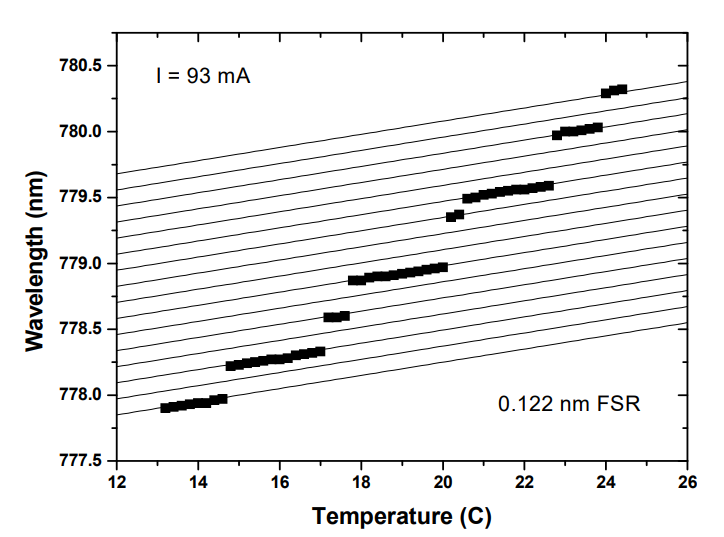
\includegraphics[width=0.8\textwidth]{ModeTemp.png}
    \caption{Einfluss der Temperatur auf das Modenspektrum und die Wellenlänge \cite{ap60}.}
    \label{fig:Temp}
\end{figure}
Wenn die Temperatur erhöht wird, hat dies einen Einfluss auf die Bandlücke sowie auf den Brechungsindex des 
Mediums. Dies beeinflusst das Modenspektrum des inneren Resonators. Da die Energiebandabstände sich stärker verändern 
als das Modenspektrum, kommt es zu Modensprüngen.
\\
\\
Auch der Pumpstrom hat einen Einfluss auf den Peak der Wellenlänge. Diese Abhängigkeit ist in \autoref{fig:Curr}
zu sehen.
\begin{figure}
    \centering
    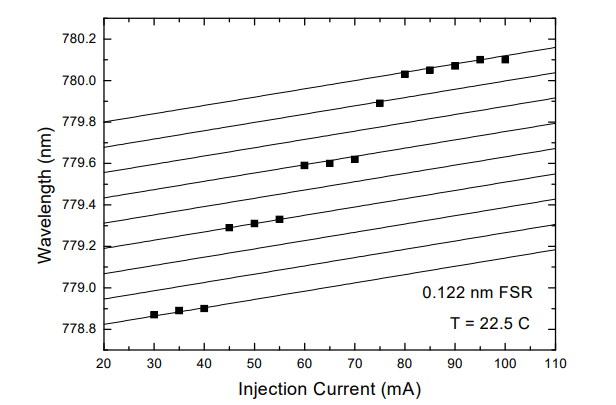
\includegraphics[width=0.8\textwidth]{ModeCurr.png}
    \caption{Einfluss des Pump-Stroms auf die Wellenlänge \cite{ap60}.}
    \label{fig:Curr}
\end{figure}
Ein erhöhter Pumpstrom führt nicht nur zu einer erhöhten Temperatur, sondern auch zu einer erhöhten 
Ladungsdichte. Auch dies hat einen Einfluss auf die Wellenlänge und es kommt erneut zu Modensprüngen.
\\
\\
Die Überlagerung der Einflüsse der einzelnen Bauteile befindet sich in \autoref{fig:GainIdeal}. 
Dabei wird die Nettoleistung des inneren Resonators als gestrichelte Linie dargestellt. Als durchgezogene 
Linie wird die Nettoleistung des Gitters und die Nettoleistung des externen Resonators überlagert. 
Das Gitter hat einen Peak bei einer einzigen Wellenlänge wie in \autoref{fig:Gain}. Die Nettoleistung des externen
Resonators sorgt für diskrete Wellenlängen; dessen Einhüllende ist die Nettoleistung des Gitters.
\begin{figure}
    \centering
    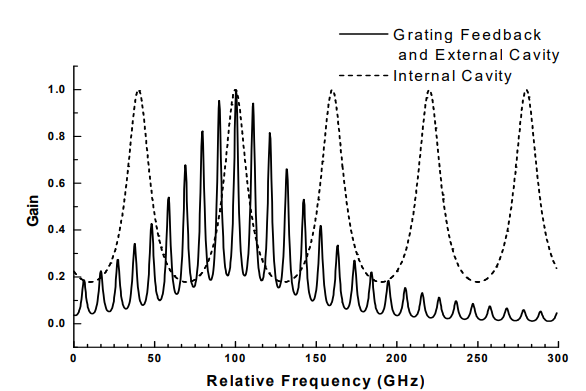
\includegraphics[width=0.8\textwidth]{CavityIdeal.png}
    \caption{Überlagerung des Einflusses des inneren Resonators, des Gitter Feedbacks und des äußeren Resonators \cite{ap60}.}
    \label{fig:GainIdeal}
\end{figure}
Dabei stimmt der Peak der Überlagerung genau mit dem Peak des inneren Resonators überein, sodass es keine Modensprünge gibt.
In \autoref{fig:ModeShifts} wird die Abhängigkeit vom Gitterwinkel dargestellt.
\begin{figure}
    \centering
    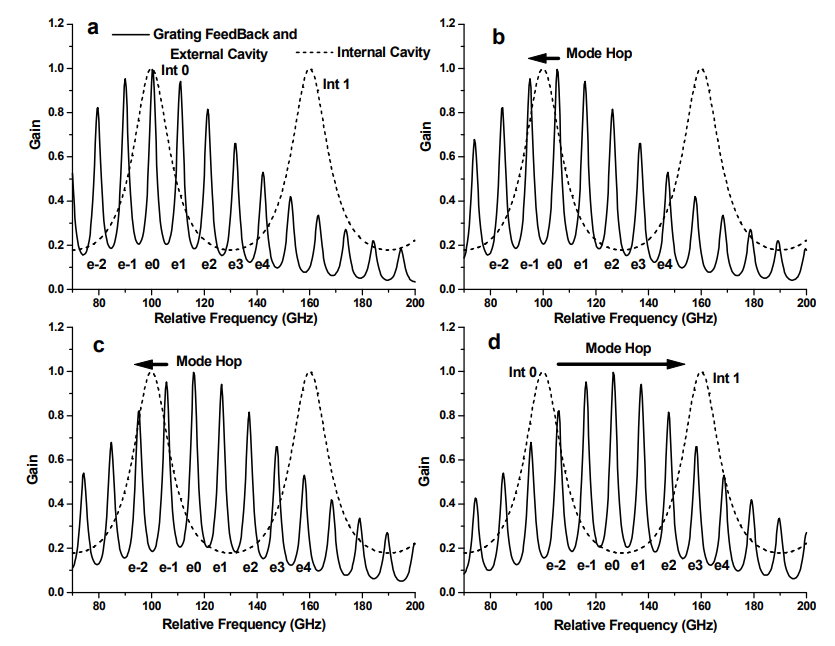
\includegraphics[width=0.8\textwidth]{ModeShifts.png}
    \caption{Einfluss der Justierung des Gitters auf das Modenspektrum \cite{ap60}.}
    \label{fig:ModeShifts}
\end{figure}
In der Abbildung a oben links befindet sich der gleiche Graph wie in \autoref{fig:GainIdeal}.
Die Moden des internen Resonators wurden mit Int0 und Int1 beschriftet, die Moden des externen Resonators werden mit e-2, e-1, ..., e4
bezeichnet. In Abbildung a befindet sich die Mode e0 genau unterhalb von Int0
Nun wird der Gitterwinkel reduziert, wodurch die Moden des externen Resonators zu einer höheren Frequenz verschoben werden. 
In Abbildung b oben rechts wurde der Gitterwinkel soweit reduziert, dass die Mode Int0 sich genau mittig zwischen den Moden e-1 und e0 befindet. 
Dies führt zu einem Modensprung zu der Mode e-1. Wenn der Gitterwinkel nun weiter reduziert wird, verschieben sich die Moden des externen Resonators weiter zu 
höheren Frequenzen. In Abbildung c findet entsprechend ein Modensprung zu e-2 statt. In Abbildung d unten rechts wurde der Winkel 
so weit reduziert, dass die Mode e3 des externen Resonators genau mittig unter der Mode Int1 des inneren Resonators liegt. Dies führt 
zu einem großen Modensprung zu der Mode e3.

\subsection{Absorptionsspektrum von Rubidium}
Auf der rechten Seite von \autoref{fig:RbSpectrum} ist das zu erwartende Spektrum von Rubidium dargestellt. Dieses wird durch Abfälle der Leistung
der transmittierten Strahlung dargestellt. Die Energieniveaus der beiden Isotope von Rubidium sind links in der Abbildung zu sehen. Die 
Energieniveaus liegen dicht beieinander.
\begin{figure}
    \centering
    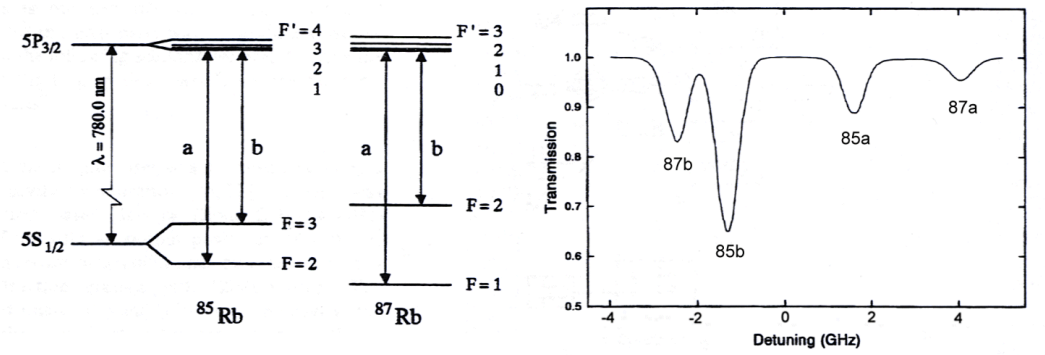
\includegraphics[width=0.9\textwidth]{SpectrumIdeal.png}
    \caption{Spektrum von Rubidium \cite{ap60}.}
    \label{fig:RbSpectrum}
\end{figure}
\section{Aufbau}
\label{sec:Aufbau}


\section{Durchführung}
\label{sec:Durchführung}

\sectiuon{Implementation}
\label{sec:implementation}
This experiment uses a diode laser as a source of coherent light. The light can be adjusted by a turning a screw that changes the angle of a diffraction grating. 
In addition to that, a so called collimator is used to narrow the emitted light to a smaller, more precise beam 


\subsection{Rubidium Flourescence and its spectrum}
\label{sec:Rubi}
For the study of Rubidium's Flourescence, the experiment used for the first part of this experiment needs to be modified.
The Rubidium Cell, which is placed between Field Coils and inside a heater to control its temperature, is set up between the ND Filter Holder and the laser.
\section{Auswertung}
\label{sec:Auswertung}

%\subsection{Fehlerrechnung}
\label{sec:Fehlerrechnung}
Für die Fehlerrechnung werden folgende Formeln aus der Vorlesung verwendet.
für den Mittelwert gilt
\begin{equation}
    \overline{x}=\frac{1}{N}\sum_{i=1}^N x_i ß\; \;\text{mit der Anzahl N und den Messwerten x} 
    \label{eqn:Mittelwert}
\end{equation}
Der Fehler für den Mittelwert lässt sich gemäß
\begin{equation}
    \increment \overline{x}=\frac{1}{\sqrt{N}}\sqrt{\frac{1}{N-1}\sum_{i=1}^N(x_i-\overline{x})^2}
    \label{eqn:FehlerMittelwert}
\end{equation}
berechnen.
Wenn im weiteren Verlauf der Berechnung mit der fehlerhaften Größe gerechnet wird, kann der Fehler der folgenden Größe
mittels Gaußscher Fehlerfortpflanzung berechnet werden. Die Formel hierfür ist
\begin{equation}
    \increment f= \sqrt{\sum_{i=1}^N\left(\frac{\partial f}{\partial x_i}\right)^2\cdot(\increment x_i)^2}.
    \label{eqn:GaussMittelwert}
\end{equation}
\subsection{Bestimmung des Schwellenstroms}
\label{sec:Ausw1}
Zur Bestimmung des Schwellenstroms wird wie in \autoref{sec:AufbLasergran} vorgegangen. Dadurch konnte von Schwellenstrom von $34.9\,\unit{\milli \ampere}$ ermittelt werden. Die zugehörigen Bilder hierzu sind \autoref{fig:befTresh} und \autoref{fig:Boom}.

\begin{figure}
    \centering
        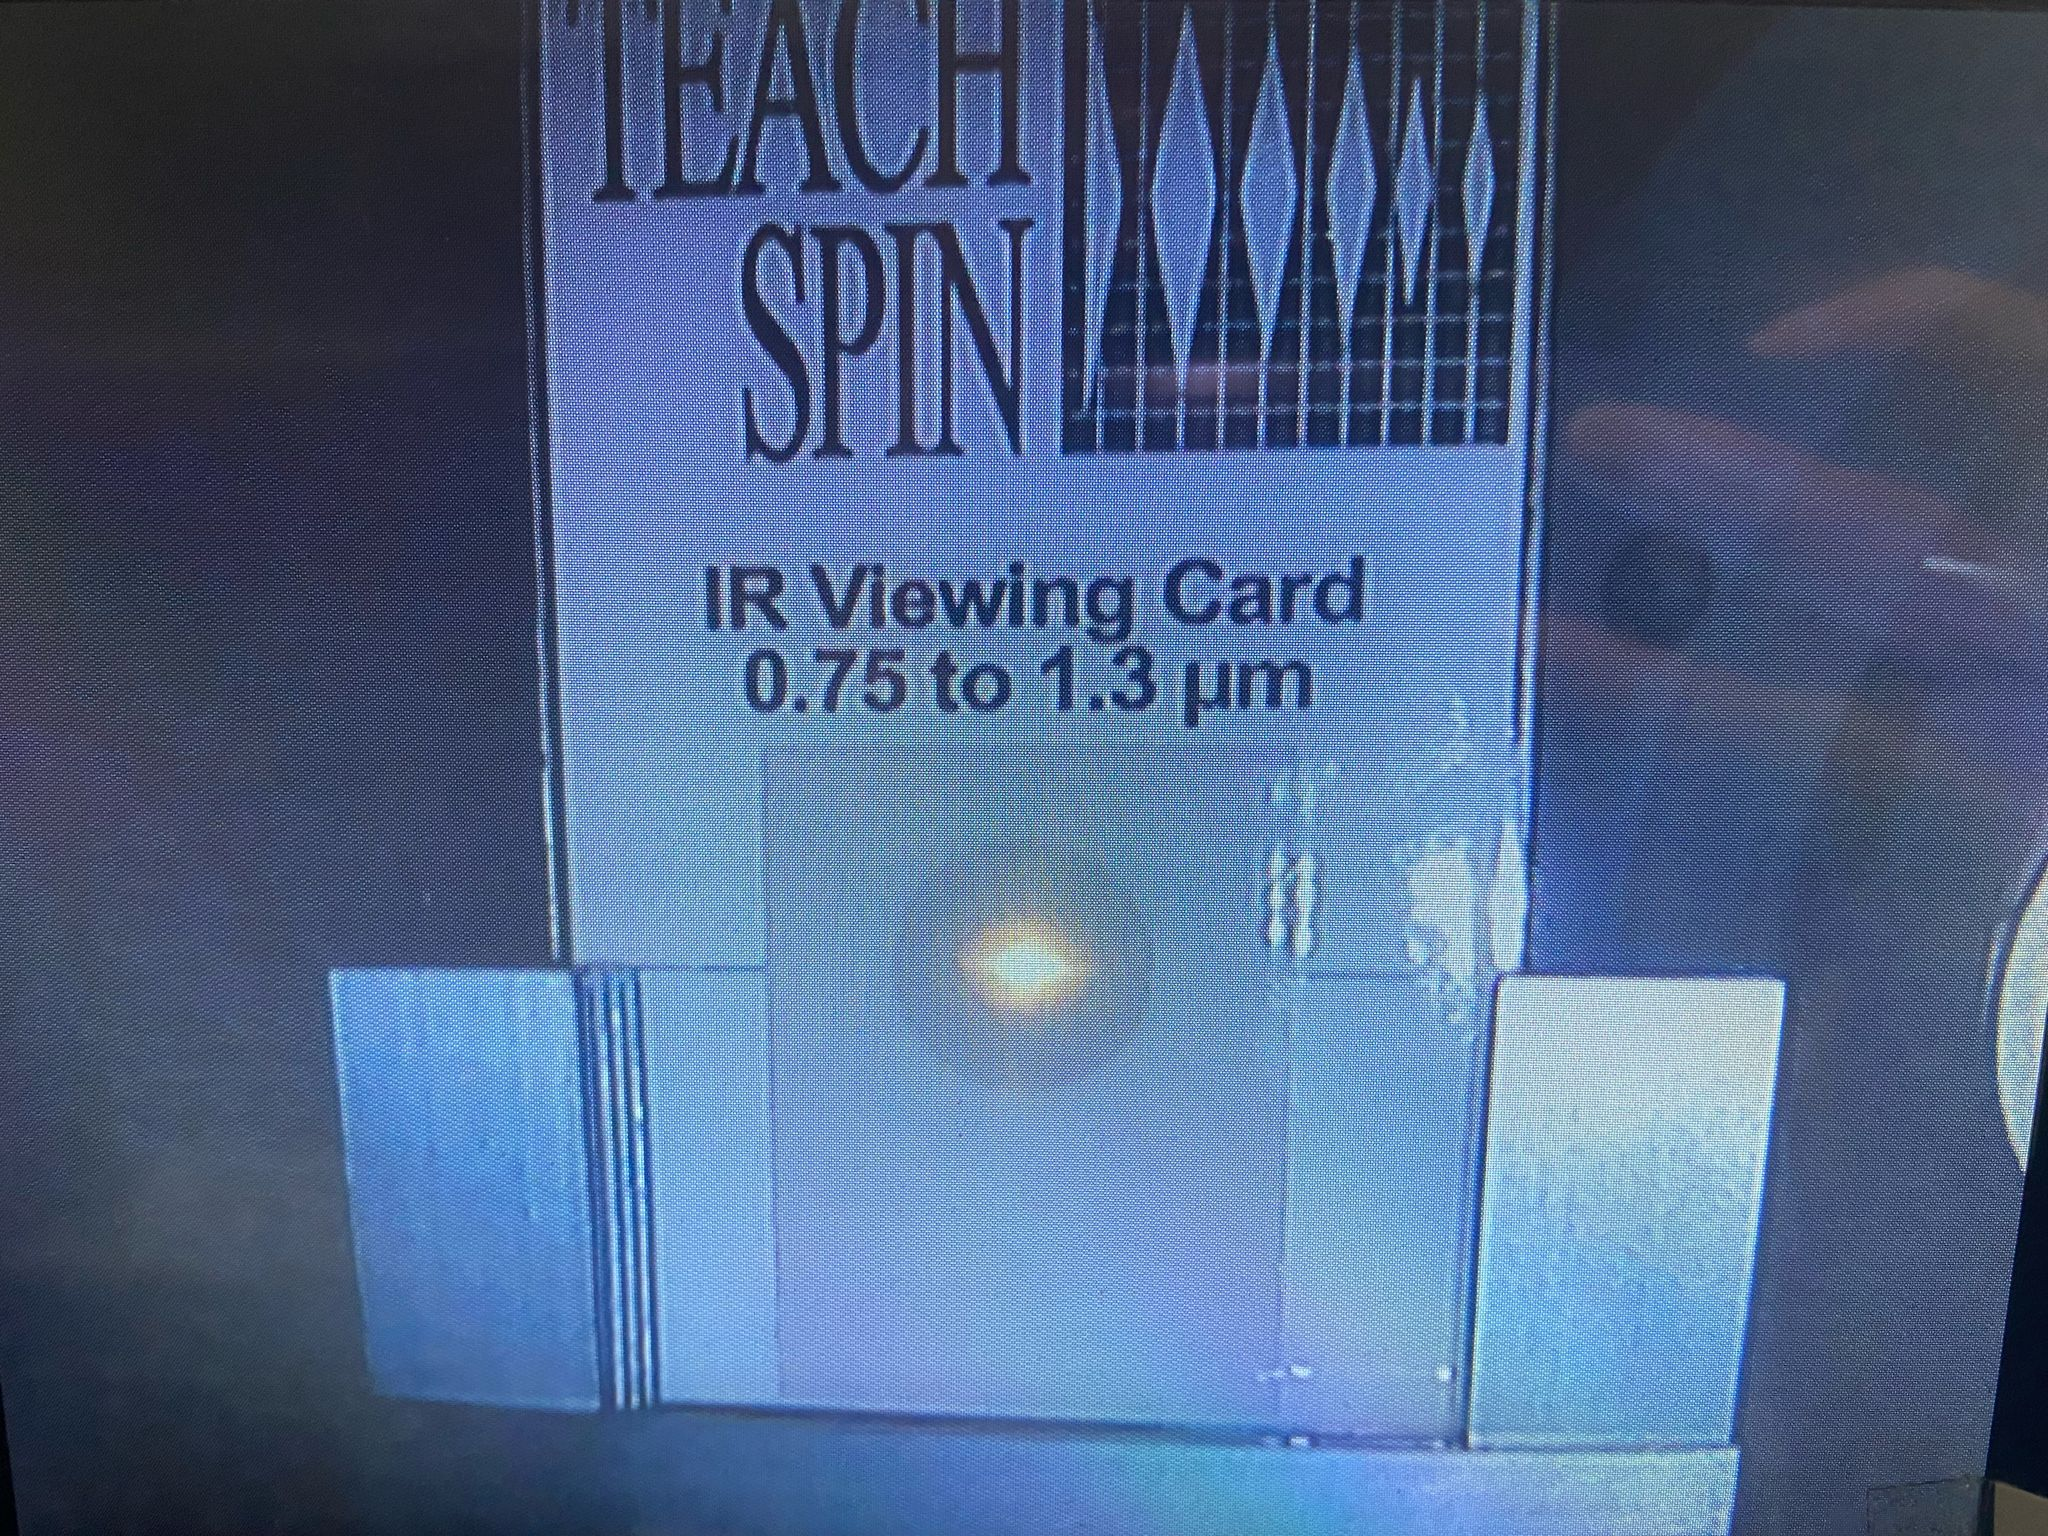
\includegraphics[width=0.8\textwidth]{beforeThreshold.jpeg}
        \caption{Lichtbild unterhalb des Schwellenstroms ($34.1\,\unit{\milli \ampere}$).}
        \label{fig:befTresh} 
\end{figure}
\begin{figure}
    \centering
        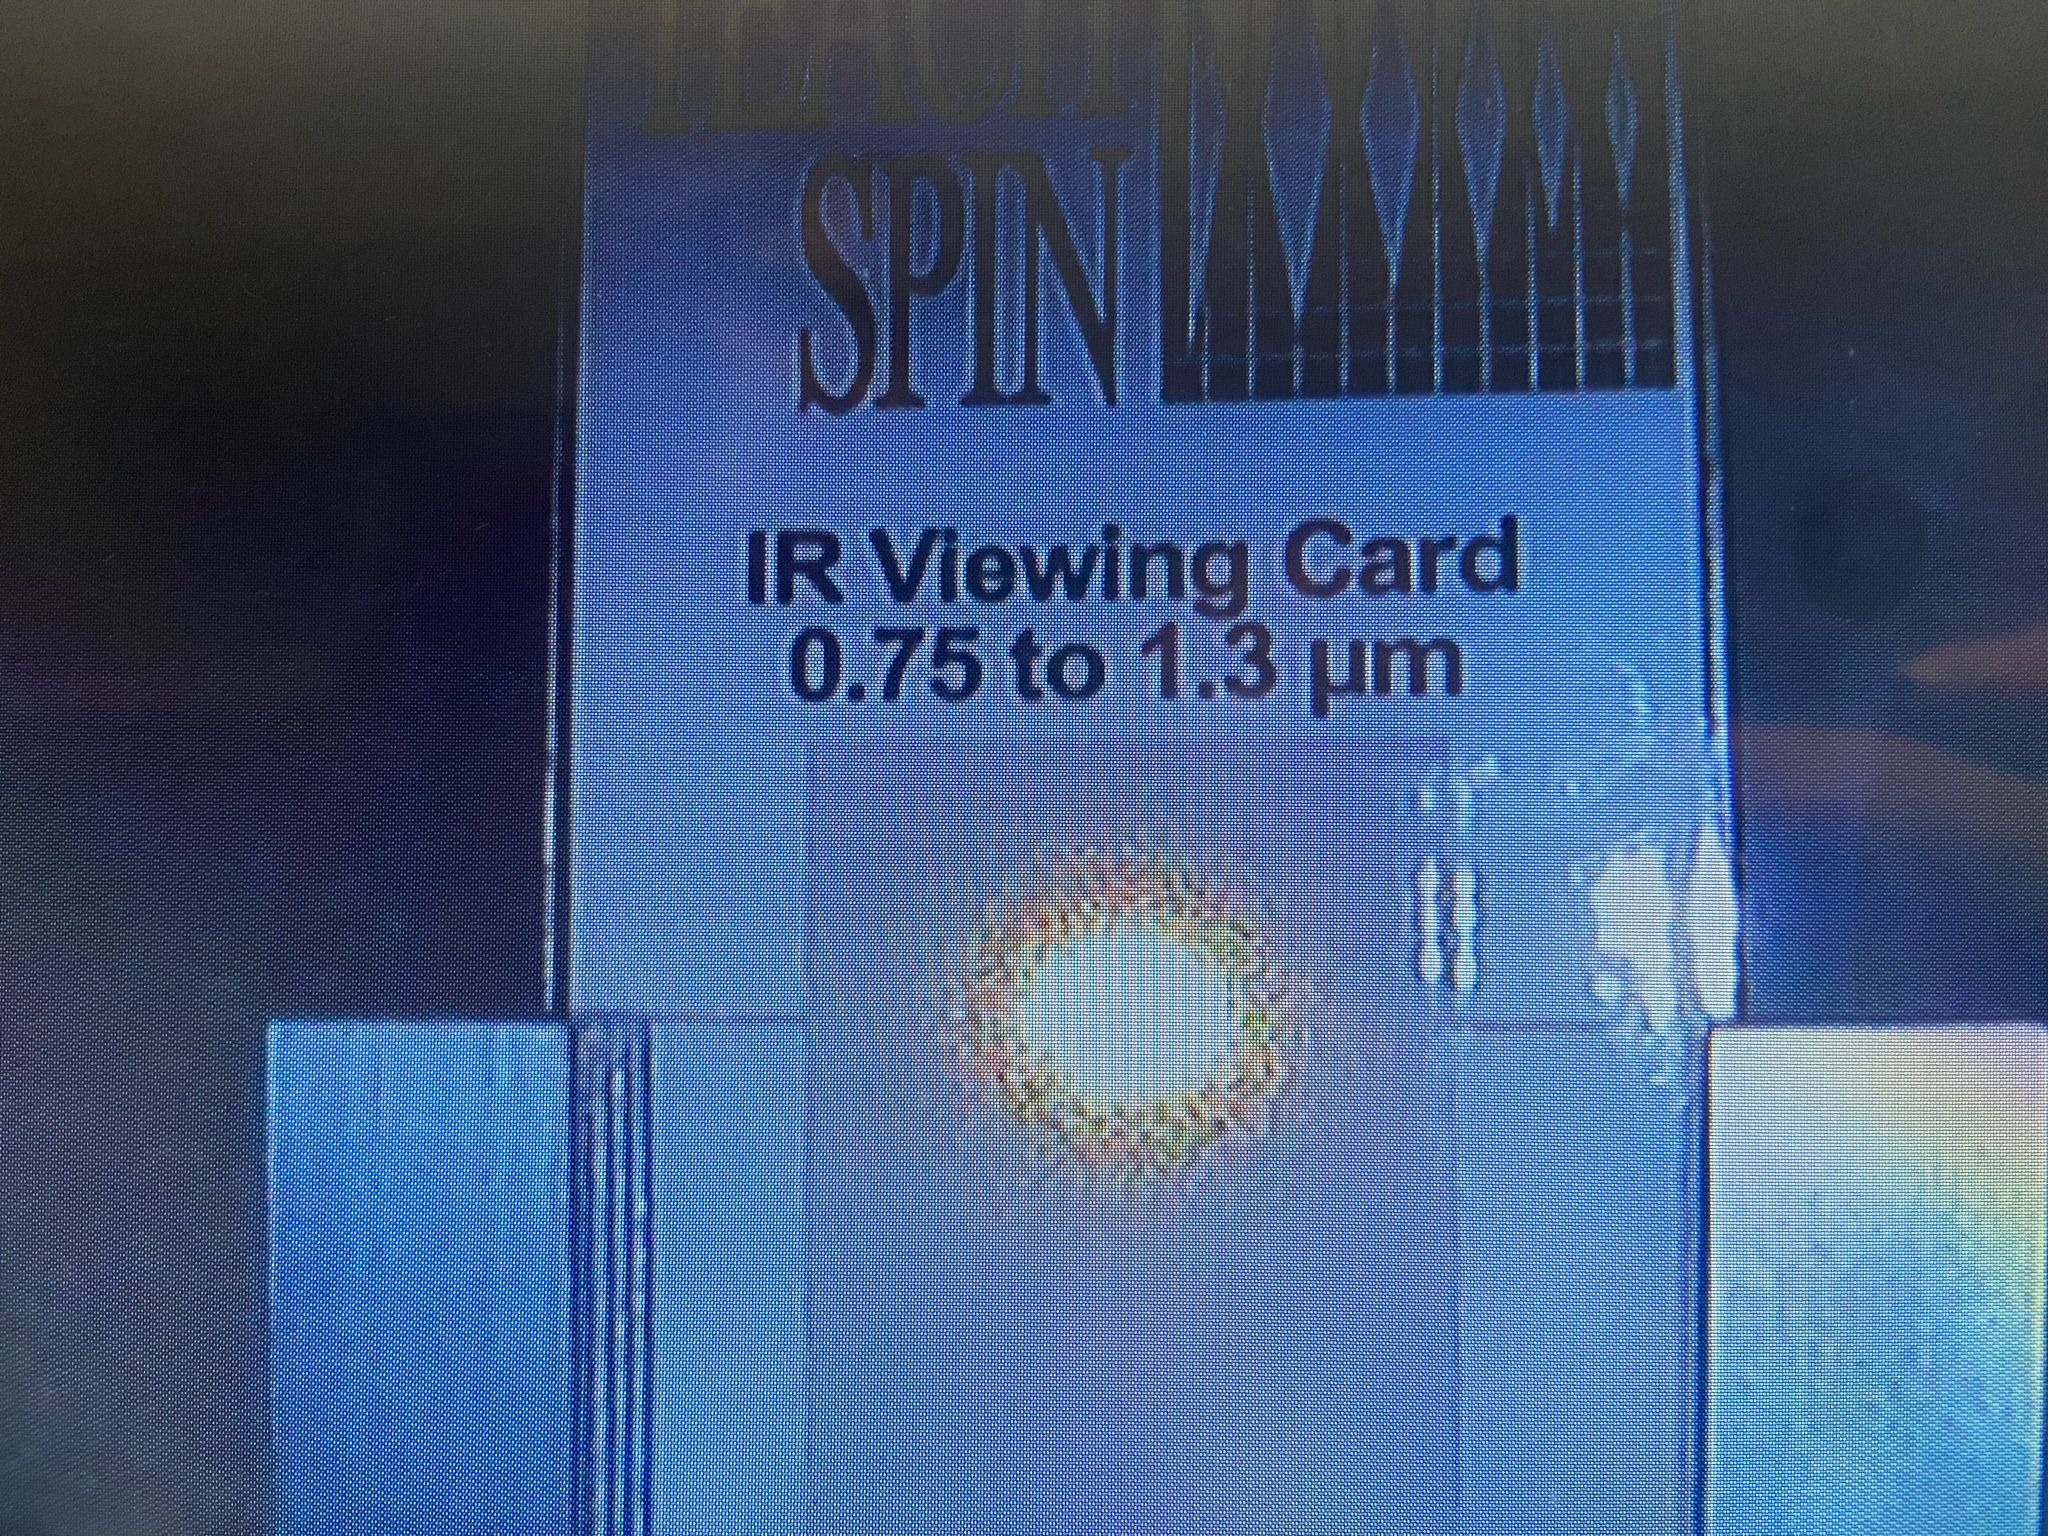
\includegraphics[width=0.8\textwidth]{Lasergranulation.jpeg}
        \caption{Lasergranulation über Schwellenstroms ($36.4\,\unit{\milli \ampere}$).}
        \label{fig:Boom} 
\end{figure}

\subsection{Rubidium-Floureszenz und dessen Spektrum}
\label{sec:Ausw2}
In \autoref{fig:Flour} ist deutlich die Linie der Floureszenz zu erkennen. Das Transmissionsspektrum ist in \autoref{fig:Transmis} als gelbe Linie zu sehen. Hierbei sind die in \autoref{fig:RbSpectrum} gezeigten Übergänge zu sehen.

\begin{figure}
    \centering
        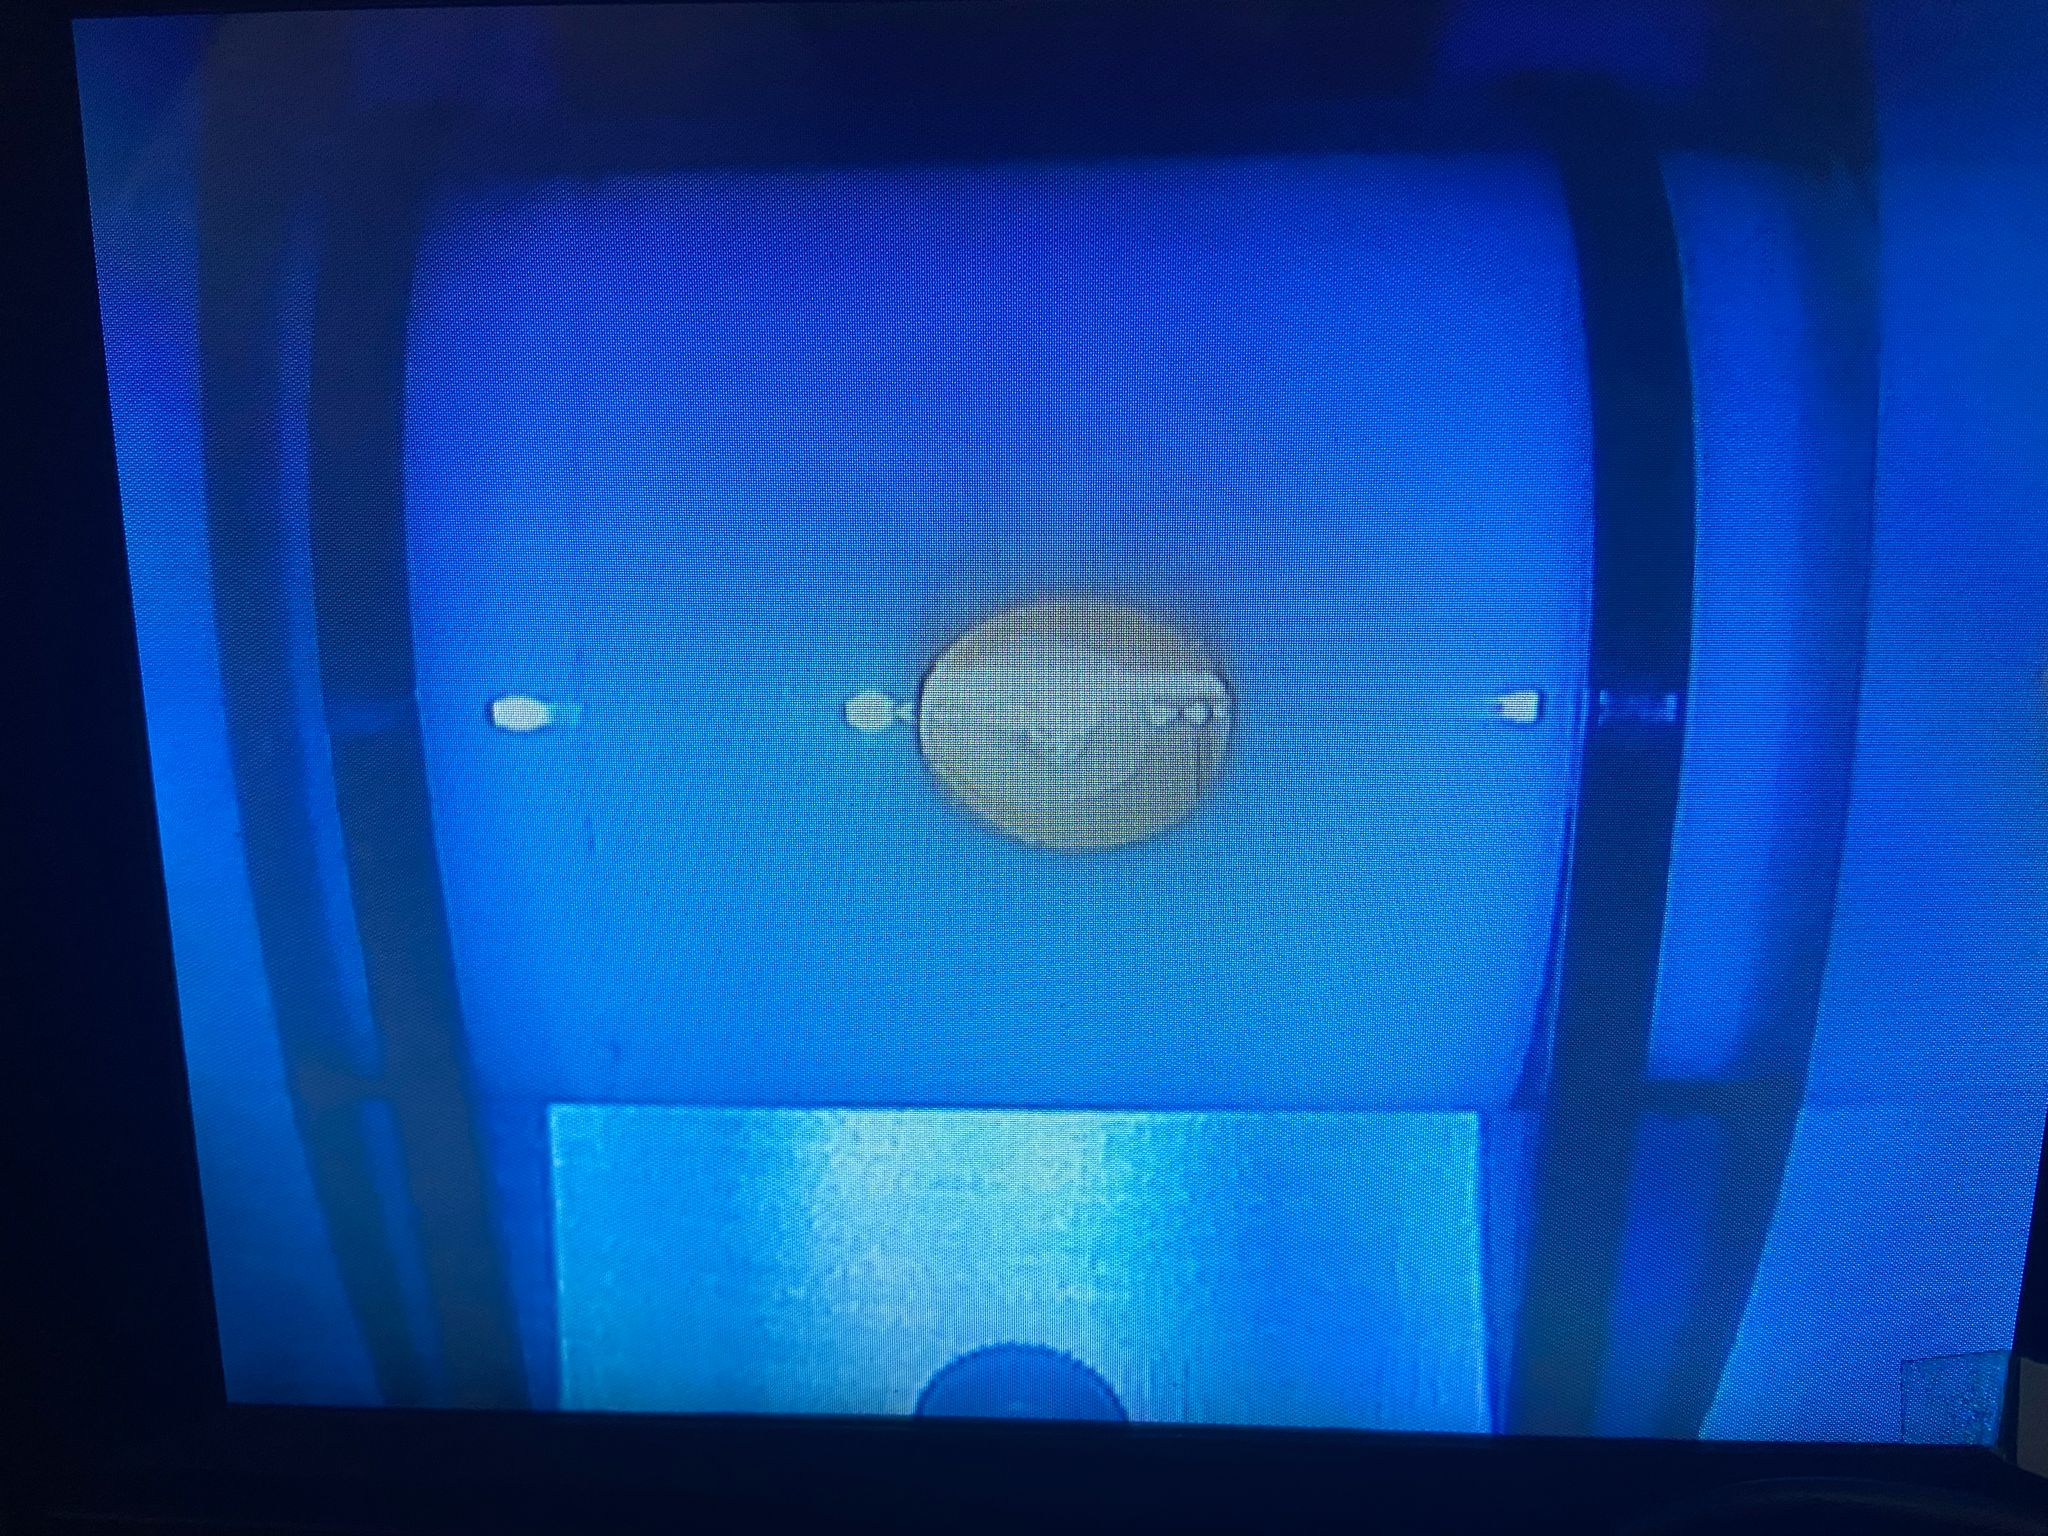
\includegraphics[width=0.8\textwidth]{Luminiszenz.jpeg}
        \caption{Floureszenz des Rubidiums.}
        \label{fig:Flour} 
\end{figure}

\begin{figure}
    \centering
        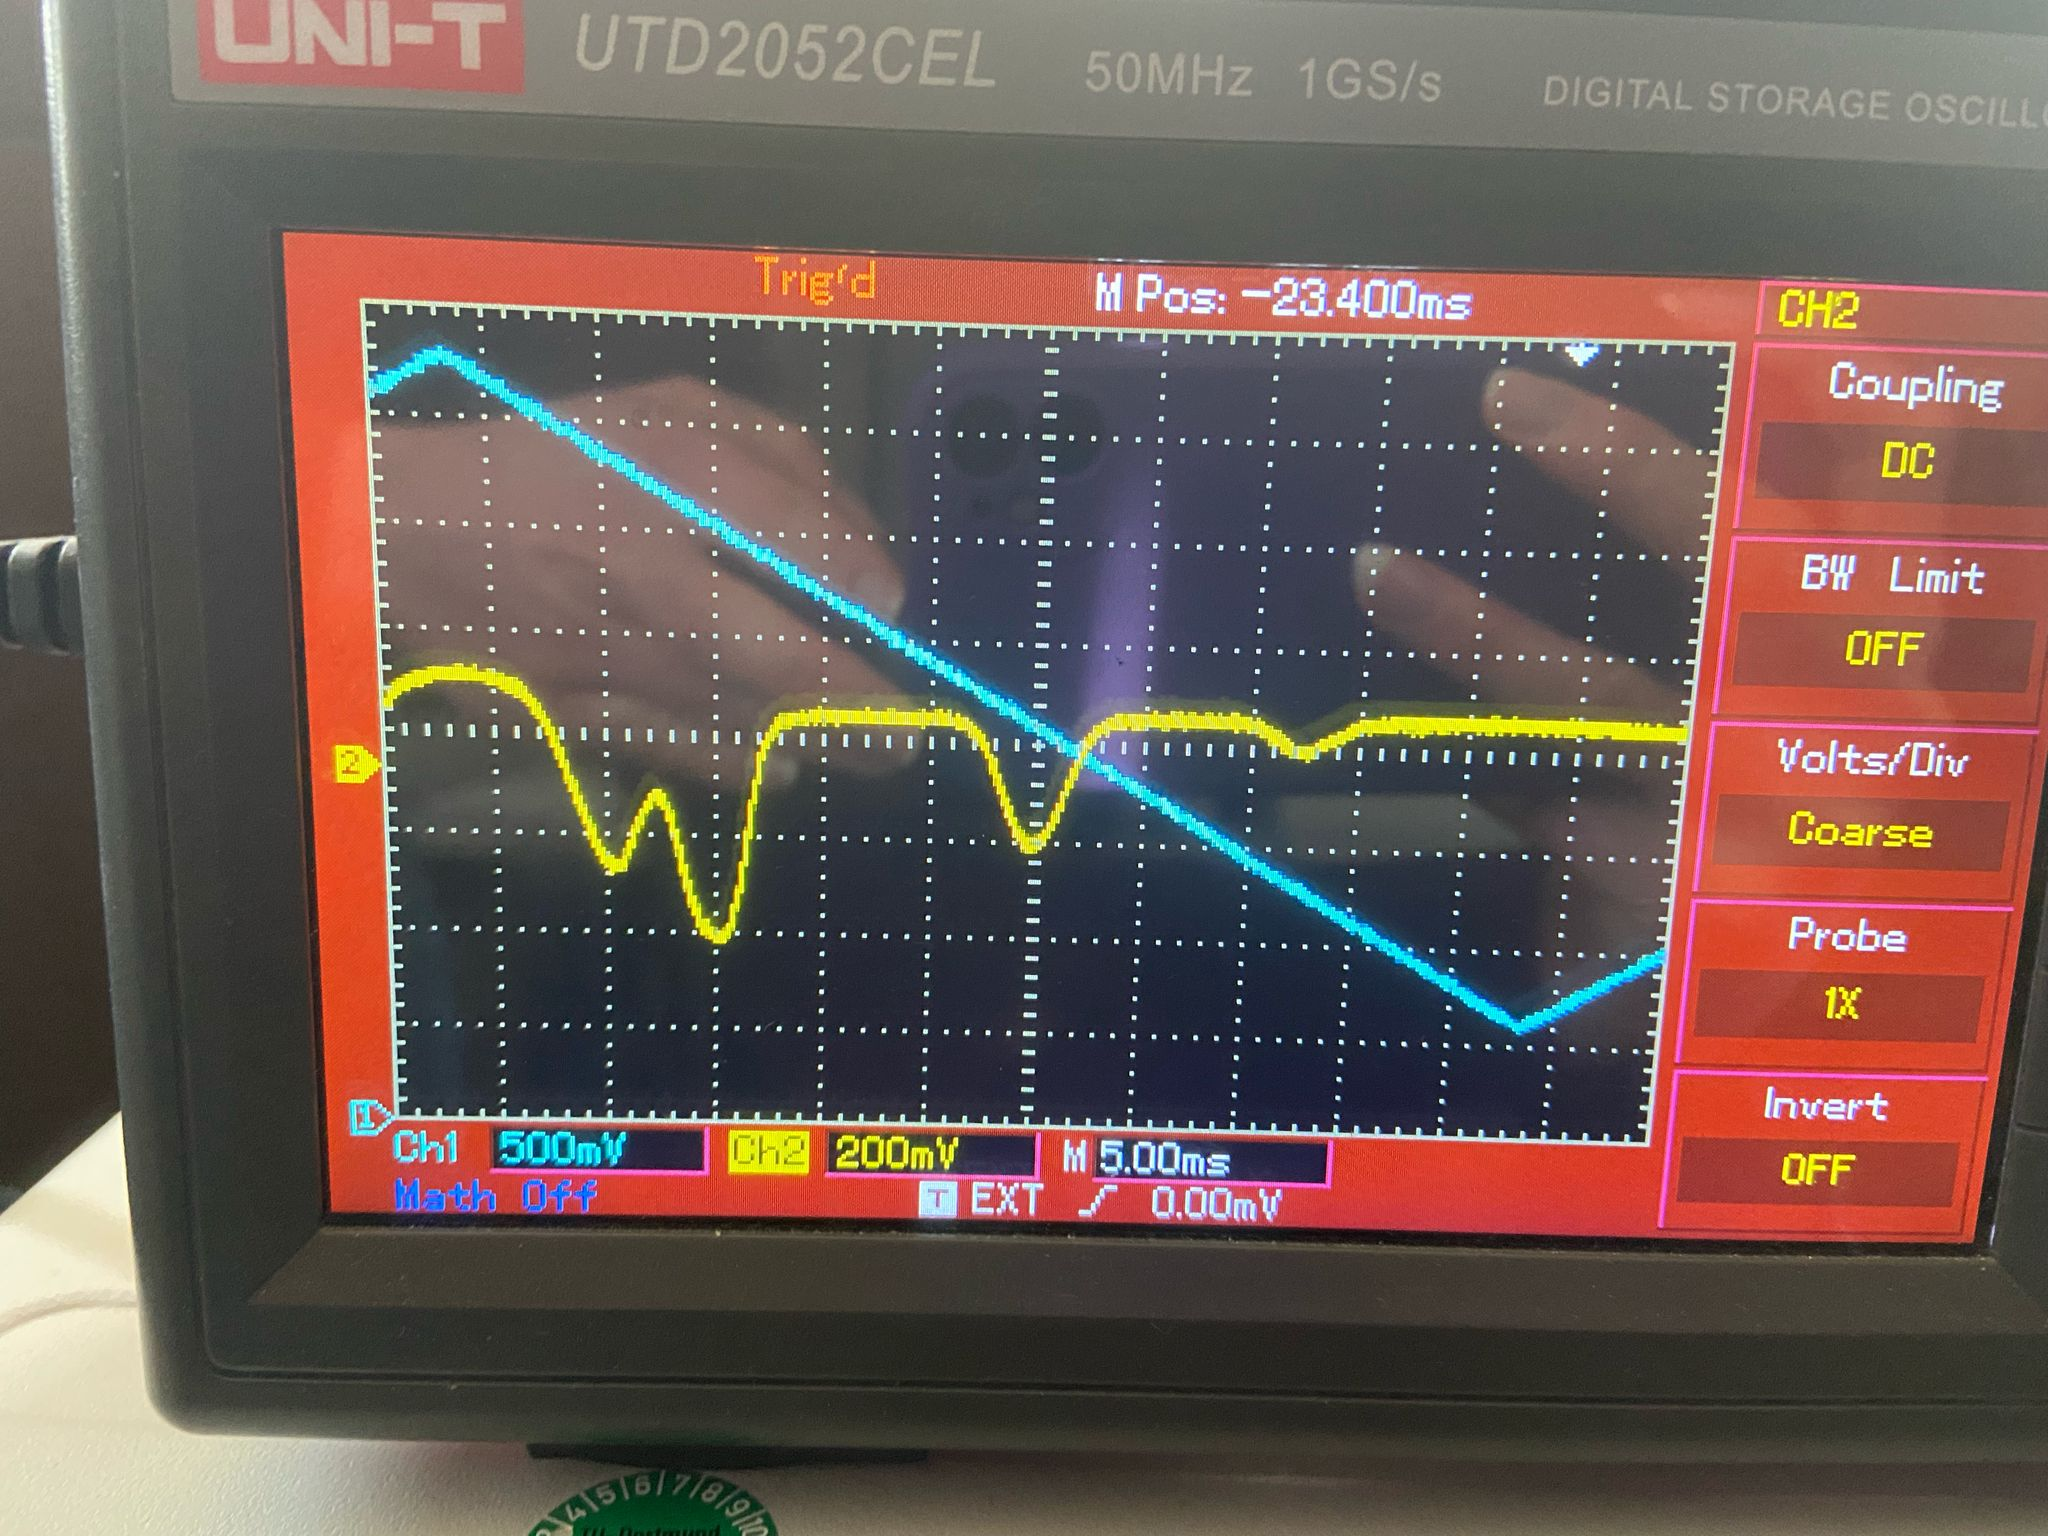
\includegraphics[width=0.8\textwidth]{Spectrum.jpeg}
        \caption{Transmissionspektrum des Rubidiums.}
        \label{fig:Transmis} 
\end{figure}
\section{Diskussion}
\label{sec:Diskussion}


\newpage
\printbibliography
\nocite{ap308}
\nocite{matplotlib}
\nocite{numpy}
\nocite{scipy}
\nocite{uncertainties}
\nocite{reback2020pandas}

\newpage
%\includepdf[scale=0.7,pages=1,pagecommand=\section*{Anhang}\thispagestyle{empty}]{messdaten.pdf}
%\addcontentsline{toc}{section}{\protect\numberline{}Anhang}
%\includepdf[scale = 0.7, pages=-]{messdaten.pdf}

\end{document}
